\subsection{Rangefinder Implementation}
With the data acquisition command set, the rangefinder needs to be connected to the ZedBoard. Since the URG-04LX uses UART communication, there are a few reasonable options to create a UART controller on the ZedBoard.

\subsubsection{UART Options}
The ZedBoard has a few different options for controlling UART. UART can be controlled through linux, through a MicroBlaze soft-core processor, or through the Zynq-7000 Processing System. Running linux only for the purpose of using it as a UART controller would be a waste of the ZedBoard's valuable resources, as linux provides extreme capability. The MicroBlaze soft-core processor would be a better alternative, but it runs in the programmable logic in the FPGA and is unnecessary when the ARM processor on the ZedBoard is unused \cite{microblaze}. Because of this, we decided to utilize the ARM processor on the ZedBoard by using the Zynq7 Processing System via Xilinx's Zynq-7000 Processing System Intellectual Property (IP) core.

\subsubsection{Zynq7 Processing System}
\label{zynq7processingsystem}
The ZedBoard SoC features a dual-core ARM Cortex-A9 MPCore processing system and Xilinx Programmable Logic. The Zynq7 Processing System IP core acts as a logic interface that integrates the Programmable Software (PS) with the Programmable Logic (PL), which allows access to both on-chip and external memory interfaces, to PL clocks, to many I/O peripherals, and even to extended I/O peripherals \cite{zynq7ps}. With all of this overwhelming functionality, the processing system is easy to customize, featuring a simple user interface, once it is added into a project's block design. The user interface can be used to change the processing system's activated features. Figure \ref{zynq7ps_pic} shows the processing system customization window.

\begin{figure}[H]
	\centerline{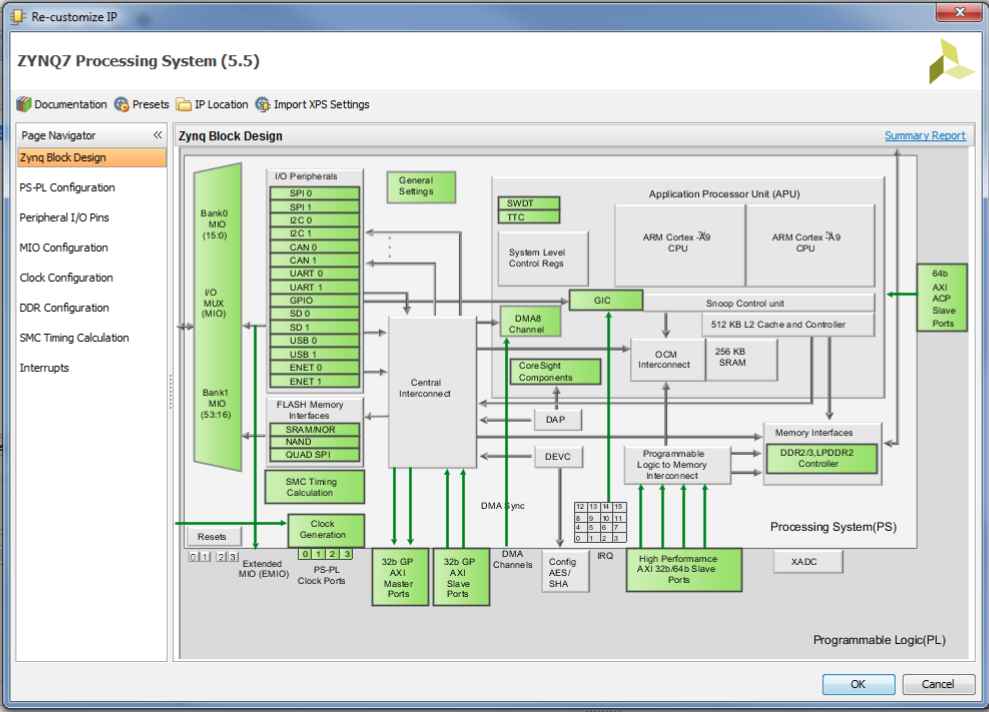
\includegraphics[width=1\textwidth]{zynq7ps.png}}
	\caption{Zynq7 Processing System Customization Window \cite{zynq7ps}}
	\label{zynq7ps_pic}
\end{figure}

In the figure above there are two options for UART shown: UART0 and UART1. The functionality of UART0 and UART1 are nearly identical, except that UART1 has the capability of being routed to the ZedBoard's USB UART port, which is not compatible with the rangefinder \cite{zedboard_datasheet}. So, we arbitrarily chose UART0 and routed the signals to MIO10 and MIO11, which correspond to the ZedBoard's PS Pmod, JE.
\par
After choosing UART0 and configuring the MIO pins, the baud rate needs to be configured such that it corresponds with the rangefinder's default communication speed, 19200 baud \cite{urg04lx_datasheet}. This can be done in the processing system's customization window under PS-PL Configuration on the sidebar in Figure \ref{zynq7ps_pic}. Figure \ref{zynq7ps_baud_pic} shows the PS-PL Configuration window.

\begin{figure}[H]
	\centerline{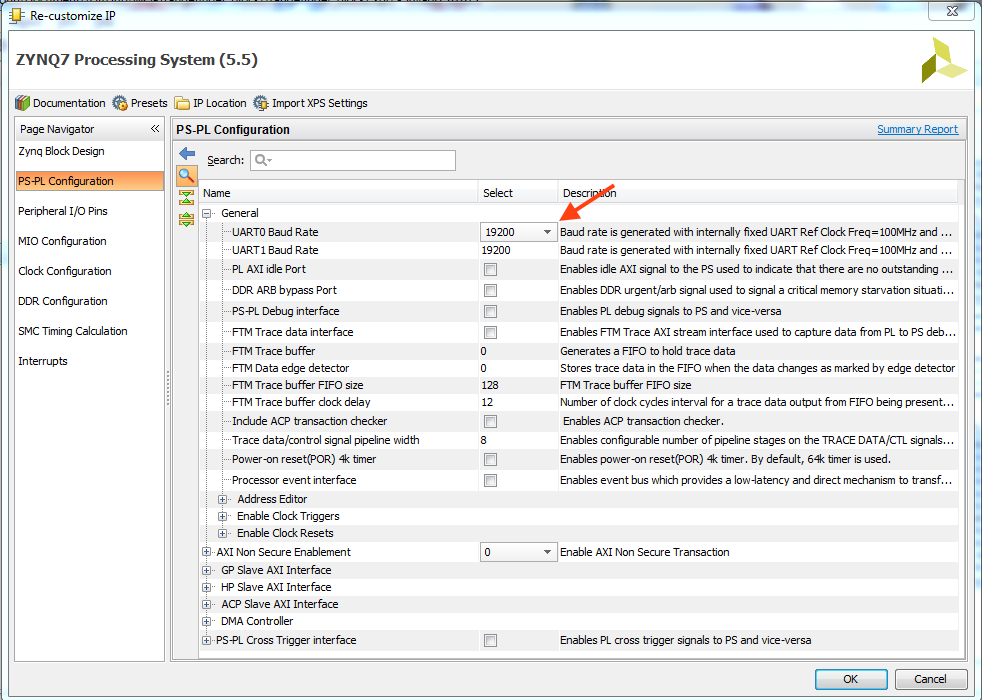
\includegraphics[width=1\textwidth]{zynq7ps_baud.png}}
	\caption{Zynq7 Processing System PS-PL Configuration Window}
	\label{zynq7ps_baud_pic}
\end{figure}

With the processing system customized in this fashion, the Programmable Logic's configuration is complete.

\subsubsection{Designing with the Xilinx SDK}
The Programmable Software (PS) is coded in the Xilinx SDK, and can be edited in the project through Vivado. To launch the SDK, the design must be exported. This is done by generating a bitstream. The bitstream compiles all the project's customization into a $.bit$ file which is used to program the FPGA on the ZedBoard. Generating a bitstream can be done in Vivado under the Program and Debug section of the Flow Navigator, as seen in Figure \ref{generateBitstream}.

\begin{figure}[H]
	\centerline{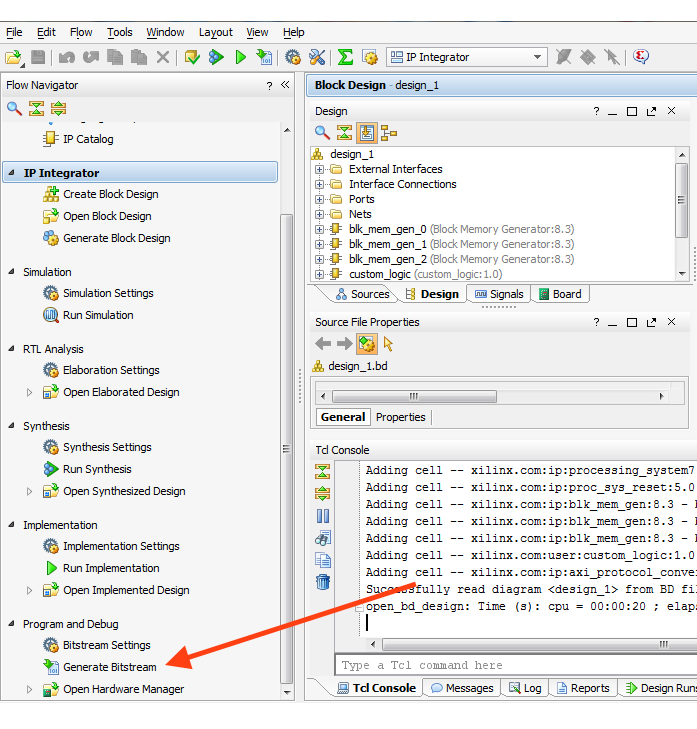
\includegraphics[width=.85\textwidth]{generateBitstream.png}}
	\caption{Generating a Bitstream in Vivado}
	\label{generateBitstream}
\end{figure}

Once the bitstream is generated, the hardware needs to be exported to the SDK so that the PS has platform to be coded on. This done in Vivado by choosing File $\rightarrow$ Export $\rightarrow$ Export Hardware and including the bitstream. Finally, the SDK can be launched by choosing File $\rightarrow$ Launch SDK.
\par
When the SDK launches, there will be a hardware platform project in the Project Explorer tab. This file contains the hardware platform that was exported from Vivado and will be used to program the FPGA on the ZedBoard. To begin programming the PS, an Application Project must be created with the hardware platform. In the SDK, choose File $\rightarrow$ New $\rightarrow$ Application Project. Enter a project name and choose Next. Note that the hardware platform exported from Vivado is selected in the Hardware Platform and is used to create the Application Project. Next, a template can be chosen to begin designing. For this project, the 'Hello World' template was chosen. This process is shown in Figure \ref{newApplicationProject}. The new Application Project exists under the Project Explorer tab, and the PS can be edited in the project's source file folder.

\begin{figure}[H]
	\centerline{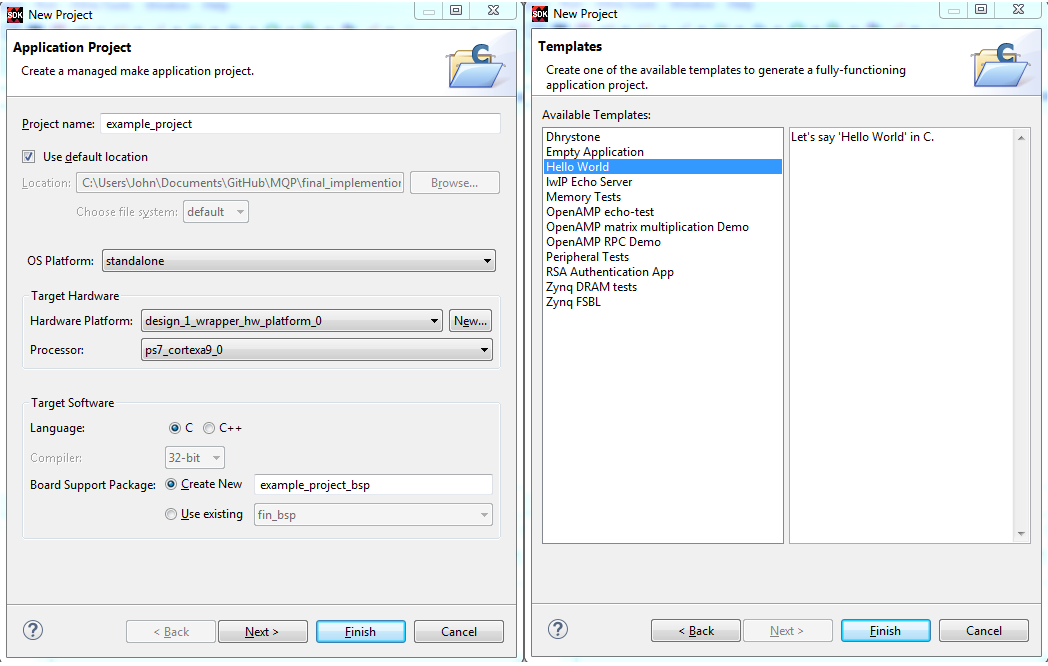
\includegraphics[width=1\textwidth]{newApplicationProject.png}}
	\caption{Creating a New Application Project in the Xilinx SDK}
	\label{newApplicationProject}
\end{figure}

When ready to program the ZedBoard, the FPGA needs to be programmed first in order to configure the PL by the hardware platform. This is done by choosing Xilinx Tools $\rightarrow$ Program FPGA. To indicate success, the ZedBoard's blue $DONE$ LED, LD12, will illuminate. Once that process has completed, the PS can be uploaded by right clicking on the application project $\rightarrow$ Run As $\rightarrow$ Launch on Hardware (GDB).



